\newSec[ControlPosAccel]{Erzeugung von Posen aus Beschleunigungsdaten}{2}




\newSec[ControlPosAccelCalc]{Berechnung}{3}
Für die nchfolgend beschriebene Berechnung der Position einer Pose wird angenommen, dass die Orientierung des \Quad[s] bekannt ist.
Es ist zu berücksichtigen, dass die Beschleunigungssensorik fest im \Quad\ verbaut ist. Der resultierende Kraft-Vektor ist in ein Koordinatensystem zu transformieren, dessen xy-Ebene parallel zu der Start-Orientierung des \Quad[s] ausgerichtet ist. \missing[Quelle?]

Anschließend kann der Kraft-Vektor entlang der Achsen des \Quad-Koordinatensystems aufgeteilt werden und die Beschleunigungen auf den \Quad\ zweifach integiert werden. Dieses Vorgehen gelingt lediglich bei idealen Daten. Da in Störungen auf das Signal wirken können, sind geeignete Methoden der Signalverarbeitung anzuwenden. \missing[Quelle?]


\newSec[ControlPosAccelDisturb]{Signalaufarbeitung}{3}
Nachfolgend soll auf die Einflüsse einer Messung eingegangen werden, welche sich die Qualität der ermittelten Pose auswirkten. Hierzu werden verschiedene Störgrößen am Beispiel eines Szenarios betrachtet und mögliche Gegenmaßnahmen gezeigt.

An dieser Stelle sei angemerkt, dass bei dem Vorgehen der Ansatz für online-Datenverarbeitung genutzt wurde. Hierbei fließen ausschließlich Daten ein, welche maximal den aktuell betrachteten Zeitstempel aufweisen.


\newSec[ControlPosAccelSzenario]{veranschaulichendes Szenario}{4}
Im gewählten Szenario wir die z-Achse \bzw\ Flughöhe als Beispiel betrachtet. 
Die Kurve setzt sich aus idealisierten Teilstücken zusammen (siehe \refImg{fig:SzeneOrigin}, oben):
\begin{itemize}
\item Initialisierung: horizontale Gerade
\item Abflug: negativer Cosinus (1/2 Schwingung)
\item Schweben: horizontale Gerade
\item Landung: zwei entgegengesetzte Parabeln\footnote{Die Parabeln sind so angeordnet, dass der Berührungspunkt zeitlich in der Mitte der Landungsphase liegt. Da die Parabeln einen identischen Streckfaktor besitzen, entspricht der Übergang zwischen den Parabeln einer knickfreien Kurve.}
\item Abschalten: horizontale Gerade
\end{itemize}


\begin{figure}[ht!]
\vspace{0.25cm}
\begin{center}
\fbox{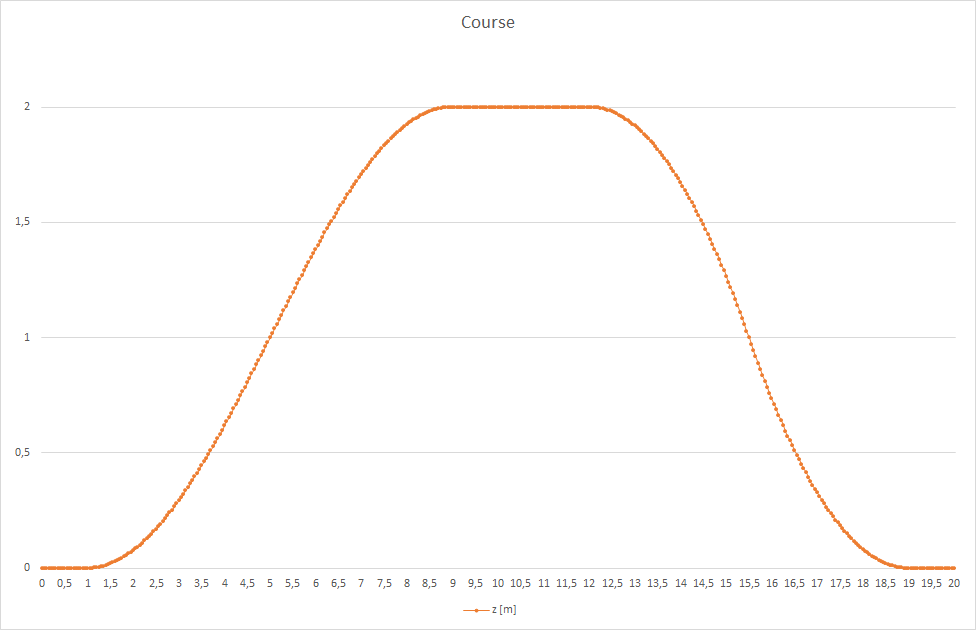
\includegraphics[width=15cm]{Pictures/Szenario Origin z.png}}
\fbox{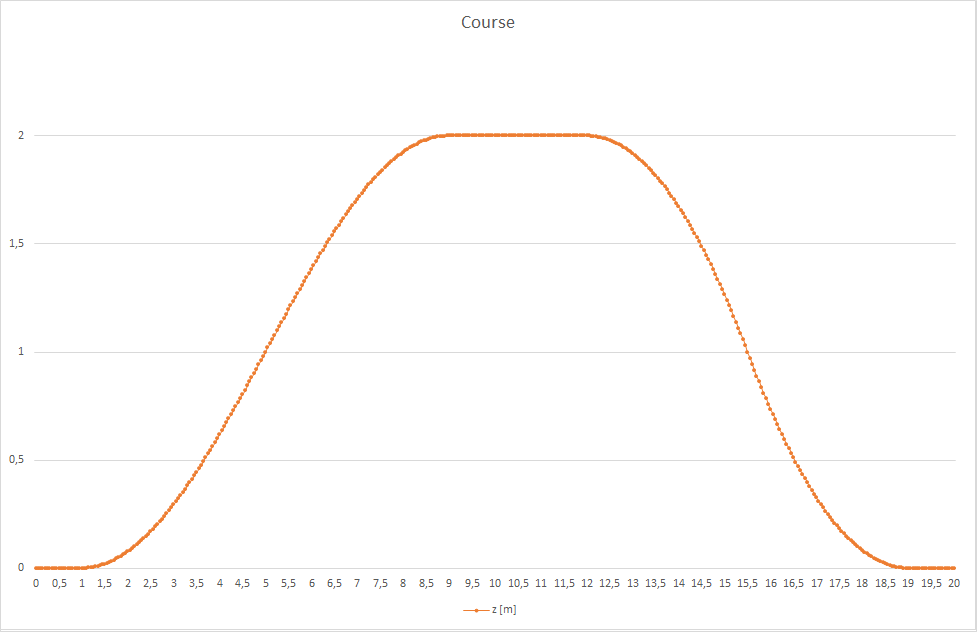
\includegraphics[width=15cm]{Pictures/Szenario Origin az.png}}
\caption{Originalkurve des Szenarios}
\label{fig:SzeneOrigin}
\end{center}

\vspace{0.25cm}
In \refImgShort{fig:SzeneOrigin} sind der idealisiete Höhneverlauf (oben) und die daraus abgeleitete Beschleunigung (unten) aufgetragen. Sofern nicht anderweitig beschrieben, wird im Folgenden eine Abtastrate von 20 Datenpunkten pro Sekunde angenommen.
\end{figure}

Die Beschleunigungsdaten wurden aus der genannten Kurve mittel zweifacher zeitdiskreter Differentation gebildet (siehe \refImg{fig:SzeneOrigin}, unten).\\
Durch dieses Vorgehen ist sichergestellt, dass ein Vergleich zwischen original Kurve und den rekonstruierten Verläufen gebildet werden kann. In diesem Zusammenhang wurde sichergestellt, dass eine Rekonstruktion ohne aufgeprägte Störgrößen möglich ist. \comp{SV1}(Seite 123)


\newSec[ControlPosAccelNoise]{Rauschen}{4}
Rauschen eines Signal kann durch die Quantisierung von analogen Daten auftreten \comp{SV1} (Seite 100, Abbildung 4.5) oder in dem Anwendungsfall einer Beschleunigungsmessung auch von Vibrationen des Systems beeinflusst werden.
Es ist darauf zu achten, dass Überläufe von digitalen Speichertypen vermieden werden, da diese einen Signifikanten Anteil an rauschenden Signalen ausmachen können. \comp{SV1} (Seite 118)

\begin{figure}[ht!]
\vspace{0.25cm}
\begin{center}
\fbox{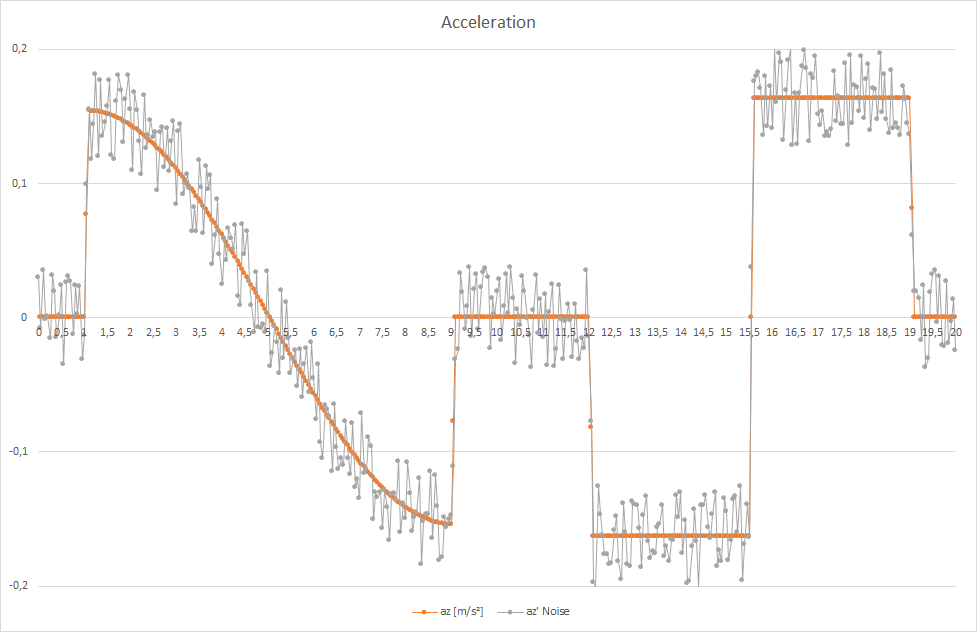
\includegraphics[width=12cm]{Pictures/Szenario Noise az.png}}
\fbox{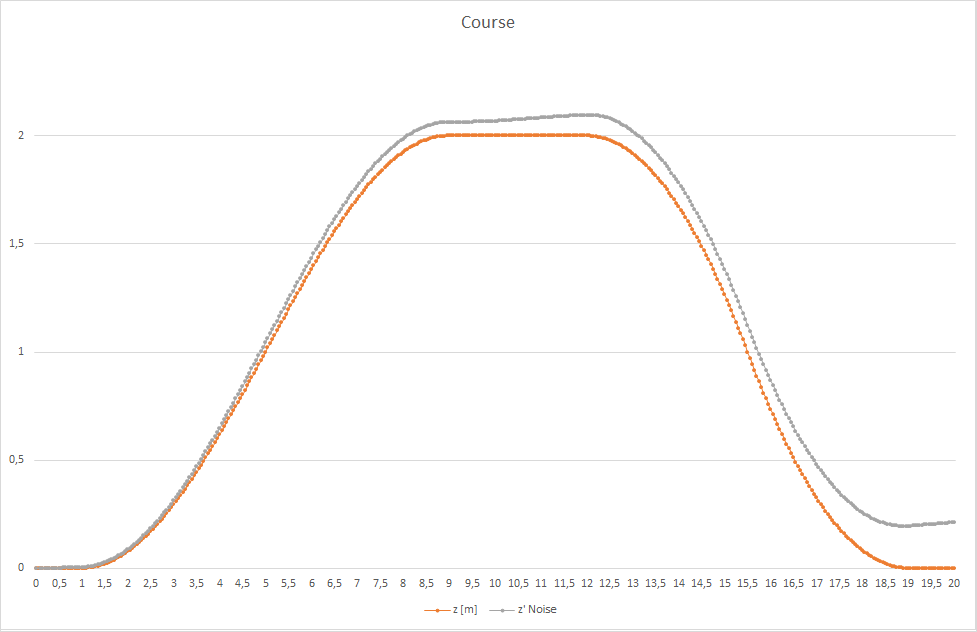
\includegraphics[width=12cm]{Pictures/Szenario Noise z.png}}
\caption{Einfluss von Signalrauschen}
\label{fig:SzeneNoise}
\end{center}

\vspace{0.25cm}
Um das aufgeprägte Rauschen zu erzeugen wurden Zufallszahlen im Bereich [-1, 1] erzeugt und diese mit dem Faktor einer angenommenen absoluten Genauigkeit (0.375\% für einen Wertebereich [-15 m/s², 15 m/s²]) und einer angenommenen relativen Genauigkeit (0.5\%) verrechnet.
\end{figure}

\missing[was dagegen tun? Eigentlich Mittelwert bilden. Aber Mittelwert glättet auch einzelne Werte. Also Höhere Abtastrate!]







\newSec[ControlPosAccelOutlier]{Ausreißer}{4}

\missing[Erklären, wie diese entstehen]

\begin{figure}[ht!]
\vspace{0.25cm}
\begin{center}
\fbox{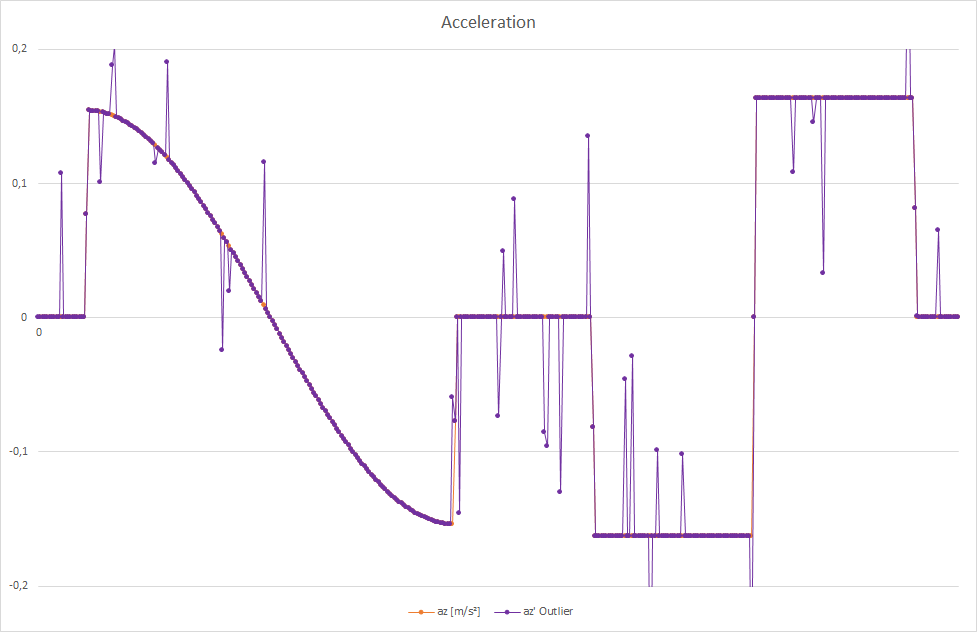
\includegraphics[width=12cm]{Pictures/Szenario Outlier az.png}}
\fbox{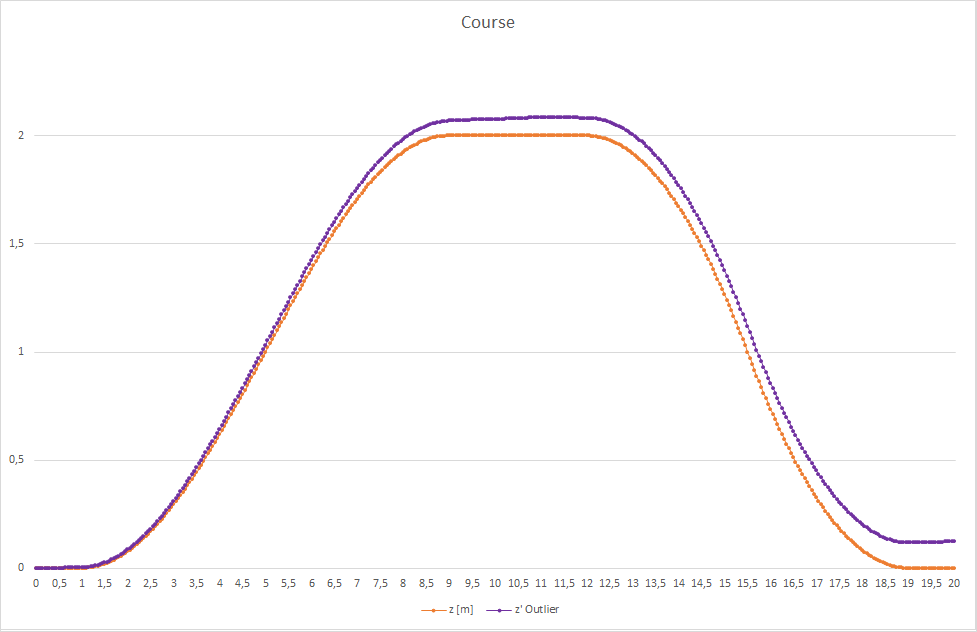
\includegraphics[width=12cm]{Pictures/Szenario Outlier z.png}}
\caption{Einfluss von Ausreißern}
\label{fig:SzeneOutlier}
\end{center}

\vspace{0.25cm}
Die Höhe der aufgeprägten Ausreißer wurde mittel einer Datenreihe von Zufallszahlen im Bereich [-1, 1], verrechnet mit dem beliebigen Faktor 0.125, generiert. Für die zeitliche Lage wurde eine Datenreihe von Zufallszahlen im Bereich [0, 1] mit einem Schwellwert von 0.925 verglichen. Daraus folgt, dass etwa 7.5\% der Datenwerte einen zusätzlichen Wert aufgeprägt bekommen.
\end{figure}


1977 wurde von Tukey beschrieben, dass ein gleitender Median für die Glättung einer Datenreihe eingesetzt werden kann \comp{DataAnalysis1}(Seite 210). Im Buch wird ein Median über drei Werte vorgeschlagen. Eine Erweitung der Anzahl der einbezogenen Werte ist möglich, wobei zu berücksichtigen ist, dass die Median-Funktion bei einer geraden Anzahl an Werten den Durchschnitt der mittleren Werte bildet.  \missing[Das ist allgemeinbildung in Mathe. Es gibt zwar ein Buch (H. Cramér, "Mathematical methods of statistics" , Princeton Univ. Press (1946) --Info von https://encyclopediaofmath.org/wiki/Median\_(in\_statistics)), aber da kommt man extrem schwer ran. reicht es, hier nur das Buch zu nennen, ohne explizite Seitenzahl?]





\newSec[ControlPosAccelOffset]{konstante Nullpunkt-Abweichung}{4}



\begin{figure}[ht!]
\vspace{0.25cm}
\begin{center}
\fbox{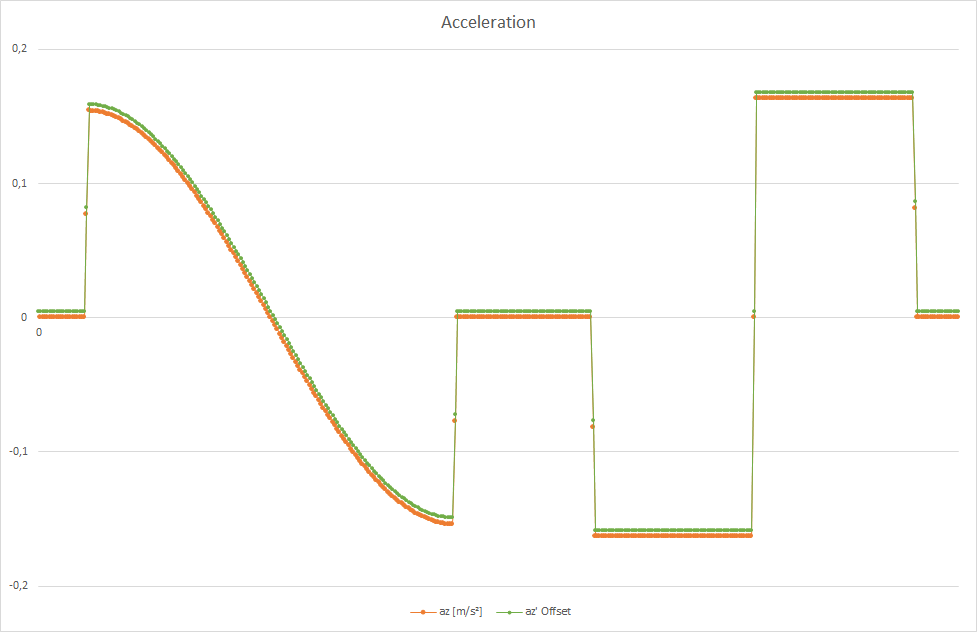
\includegraphics[width=12cm]{Pictures/Szenario Offset az.png}}
\fbox{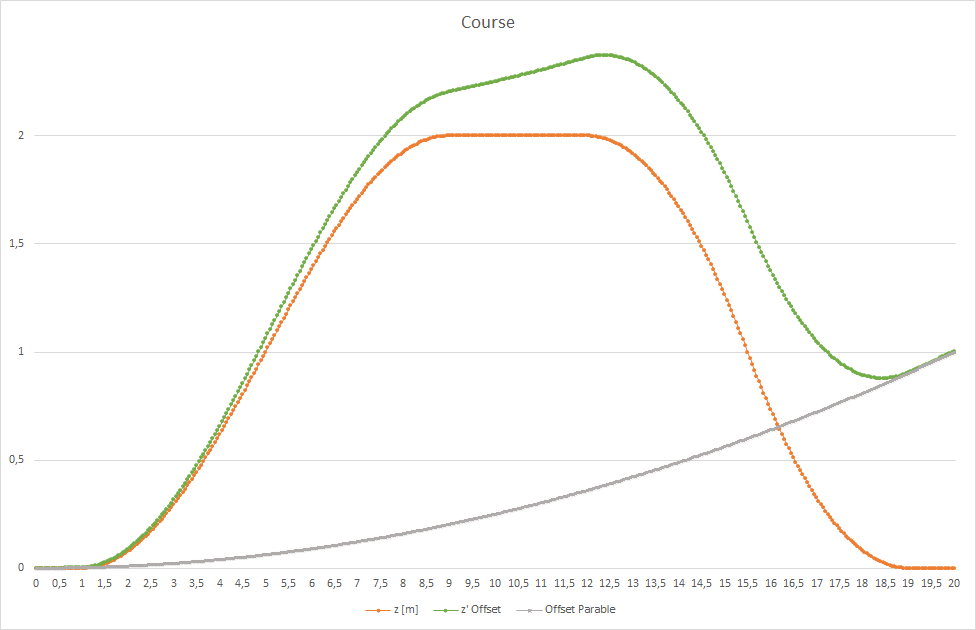
\includegraphics[width=12cm]{Pictures/Szenario Offset z.png}}
\caption{Einfluss von konstanter Nullpunkt-Abweichung}
\label{fig:SzeneOffset}
\end{center}

\vspace{0.25cm}
Die hier gezeigte Abweichung der Beschleunigungsdaten beträgt 0.0025 m/s². Die Superposition der rekonstruierten Kurve entspricht einer in grau dargestellten Parabel mit einem Streckfaktor von $\frac{\Delta a}{2}$.
\end{figure}










